\subsection{Inferring Demographics from Locations}
% We now show how location data by itself allows to infer ethnicity and gender of individual Internet users. 
% We introduce a simple frequentist approach (\S\ref{subsec:inference-algorithm}), describe considerations informing our methodology (\S\ref{subsec:method}), and present the results of its application (\S\ref{subsec:inference-results}).

% As shown above, location data from social network applications exhibit mobility patterns characterizing demographic groups. This also affects a user \emph{individually}, as location data produced by this individual are sufficiently discriminative for purposes of inferring, for example, this person's ethnicity or gender. We first develop a fundamental understanding of the problem based on a simple inference algorithm, shown optimal under strict assumptions~(\S\ref{sec:inference-algorithm}). 
% We then use traditional machine learning techniques to show that ethnicity and gender can be predicted from location data with accuracy much better than random~(\S\ref{subsec:inference-overall}).
% Next, we examine the impact of granularity and auxiliary information on our inferences~(\S\ref{subsec:inference-granularity}), finding that simple inference algorithms can be nearly as accurate as more advanced techniques. We conclude with results relating the quantity and diversity of a user's activity to our ability to make accurate predictions~(\S\ref{sec:user-activity}).

\begin{table*}[htb!]
\small
\begin{center}
\begin{tabular}{| l | c | c | c | c | c | c | c |}
\hline
\textit{Task} & \textit{Best Algorithm} & \textit{Parameters} & \textit{Important Features} & \textit{Baseline} & \textit{Accuracy} & \textit{AUC} & \textit{F1} \\ \hline
Ethnicity NY    & Log. Regression  & L1, $C=0.01$  & Avg. ZIP ethnicities & 0.52 & \textbf{0.72} & \textbf{0.76} & \textbf{0.74} \\ \hline
Ethnicity LA     & Log. Regression  & L1, $C=1$     & Avg. ZIP ethnicities & 0.50 & \textbf{0.63} & \textbf{0.66} & \textbf{0.64} \\ \hline
Gender NY & Log. Regression & L2, $C=0.1$ & Men's Store &   0.53  & \textbf{0.58} & \textbf{0.59} & \textbf{0.55} \\ \hline
\end{tabular}
\caption{Results for the binary classifications of ethnicity and gender in NY and LA. The algorithms ran on all available features, such as counts of visits to different neighborhoods, the ethnicity of the most visited block, and the categories of nearby Foursquare venues. The baseline was obtained by predicting the class of a user based on the label distribution.}
\label{tab:all-tasks}
\end{center}
\end{table*}

% \subsection{A Simple Inference Algorithm}
% \label{subsec:inference-algorithm}

% Our approach yields two advantages: (1) it provides a formulation of the problem that is intuitive and (2) it remains generic so as to be easily applicable to any sparse location dataset. We use the following assumptions: each user, $i$, belongs to one of two classes, $C_1$ or $C_2$. Class $C_1$ (respectively $C_2$) is associated with a probability distribution $\mu_1$ (respectively $\mu_2$) over a discrete set of locations, representing the fraction of time spent by users of that class in that location. Our main assumption is that a user $i$ makes $n$ checkins, denoted $X^{(i)}=(X^{(i)}_1,\ldots,X^{(i)}_n)$ at locations that are drawn independently from this user's class probability distribution. The prior probability that a user is in class $C_1$ or $C_2$ is denoted $\pi_1$ and $\pi_2$, respectively.

% Note that this model does not use notions of times of the day, geographies, or auxiliary information. It applies to most location datasets as it is agnostic to how they were generated, anonymized, or in which granularity they are available. Such model serves as a starting point to approximate human mobility~\cite{Grossglauser:2002fc}. However, in practice humans show periodicity~\cite{Gonzalez:2008wy} or even social bias~\cite{Cho:2011io} in their movements, and users in a class may not be identically distributed, which is why it is important to test our technique using real data (\S\ref{subsec:inference-results}). Under our assumptions, the problem of classifying users in their respective class reduces to a simple hypothesis testing. If $i$ is in class $C_1$ then for any location $l$, we have
% \begin{equation}
% 	\forall j%=1,\ldots,n
% 	,\;
% 	P(X^{(i)}_j=l | i\in C_1)=\mu^{(1)}(l),
% 	%\;\textrm{where}\;
% 	%\sum_{l} \mu^{(1)}(l)=1 
% 	%\;.
% \end{equation}
% \noindent so that
% \begin{equation}
% 	\resizebox{.4 \textwidth}{!}{
% 	$P(X^{(i)} = (l_1,\ldots,l_n)|i \in C_1 ) = \mu^{(1)}({l_1})  \ldots \mu^{(1)}({l_n})$,
% 	% $ P(X^{(i)} = (l_1,\ldots,l_n)|i \in C_2 ) = \mu^{(2)}_{l_1}  \ldots \mu^{(2)}_{l_n} $
% 	}
% \end{equation}
% \noindent by independence, and applying Bayes' rule
% \begin{equation}
% 	\resizebox{.4 \textwidth}{!}{
% 	$P( i \in C_1 | X^{(i)} = (l_1,\ldots,l_n) ) =
% 	%&= \frac{\pi_1 \mu^{(1)}_{l_1}  \ldots \mu^{(1)}_{l_n} }{\pi_1 \mu^{(1)}_{l_1}  \ldots \mu^{(1)}_{l_n} + \pi_2 \mu^{(2)}_{l_1}  \ldots \mu^{(2)}_{l_n}} \\
% 	\frac{1}{1 + \frac{\pi_2 \mu^{(2)}({l_1})  \ldots \mu^{(2)}({l_n})}{\pi_1 \mu^{(1)}({l_1})  \ldots \mu^{(1)}({l_n})}}$.
% 	%\;.
% 	}
% \end{equation}

% %Given a set of checkins, we wish to determine which class is more likely to have generated those checkins.
% %This is completely analogous to selecting a more likely probability distribution given a set of samples.
% %In 1933, Neyman and Pearson showed that the most powerful statistical test to resolve this is the likelihood ratio test.

% The Neyman-Pearson lemma states under the assumptions above that the most powerful statistical test to determine which class a user belongs to from its checkins is the likelihood ratio test. A maximum likelihood rule classifies a user in class 1 iff
% \begin{equation}
% 	\pi_2 \mu^{(2)}({l_1})  \ldots \mu^{(2)}({l_n}) < \pi_1 \mu^{(1)}({l_1})  \ldots \mu^{(1)}({l_n})
% \end{equation}	
% \noindent or, equivalently, if we have
% \begin{equation}
% 	\sum_{k=1}^n \ln\frac{\mu^{(1)}({l_k})}{\mu^{(2)}({l_k})} > \ln\frac{\pi_2}{\pi_1}\;.
% \end{equation}
% % Show that this is the same as the simple hypothesis test
% % Show that Neyman-Pearson should be used
% % Equations explaining this?

% We expect that our predictions are more accurate on users with more checkins. One can show under these assumptions that this classifier's error probability for a user decreases \emph{exponentially} as the number of checkins $n$ grows, that is,
% \begin{equation}
% 	P(\textrm{error} | n \textrm{ checkins}) 
% 	\approx_{n\to\infty} 2^{-n \mathcal{C}(\mu_1, \mu_2)},
% \end{equation}
% where $\mu_1$ and $\mu_2$ are the probability distributions associated with $C_1$ and $C_2$, and $\mathcal{C}$ denotes the \emph{Chernoff information}, defined as 
% \(
% \mathcal{C}(\mu_1, \mu_2) 
% = 
% -\min_{0 \leq \lambda \leq 1} \ln \sum_{l} \mu_1(l)^{1-\lambda} \mu_2(l)^\lambda\;.
% \)

% % Describe algorithm more?
% Based on this analysis, a simple algorithm to infer ethnicity or gender can first estimate $\mu_1,\mu_2$ and $\pi_1,\pi_2$ using the training data and then classify according to this likelihood rule. 


% \subsection{Methodology}
% \label{subsec:method}

% Better intro sentence
% Having shown that there exist differences between the mobile behaviors of different demographic groups, we explored if these differences were large enough for algorithms to accurately distinguish them.
% Additionally, we conducted experiments to determine the impact of granularity, auxiliary information, and quantity of data upon the accuracy of such predictions.

% Argument: provide a baseline for what can be inferred from location data
% Make methodology as generic as possible.
We now show how location data by itself allows to infer ethnicity and gender of individual Internet users.
Our purpose is to explore generally what might be inferred about users from their location data only.
This means we utilized only well-understood, and commonly applied techniques, and limited our feature sets to features derived from location data (ommitting, for example, social network features like number of followers).
We considered two questions: (1) Can minorities be distinguished from Caucasians? (2) Can women be distinguished from men?

To explore different scenarios, we respresented users as feature vectors, using three sets of features:
\textbf{geographic} features, such as counts or percentages of visits to locations; 
\textbf{semantic} features derived from Foursquare, such as the popularity of visited venues or counts of visits to venues with certain categories like ``Restaurant" or ``Park" (the collection of which we explained in \S\ref{sec:method}); 
and \textbf{Census} derived features, such as the average ethnic makeup of all visited locations or the ethnic makeup of a user's most-visited location.

We performed all our experiments using the scikit-learn library~\cite{scikit-learn} and tested the algorithms logistic regression, decision trees, naive Bayes, and support vector machines (SVMs). 
The results of our best-performing algorithms are displayed in Table~\ref{tab:all-tasks}


\paragraph{Impact of Granularity and Feature Availability}

\begin{figure*}[t]
  \centering
  % \includegraphics[width=\textwidth]{fig/last_big_plot.eps}
  \includegraphics[width=\textwidth]{fig/footprints/last_big_plot.eps}
  % 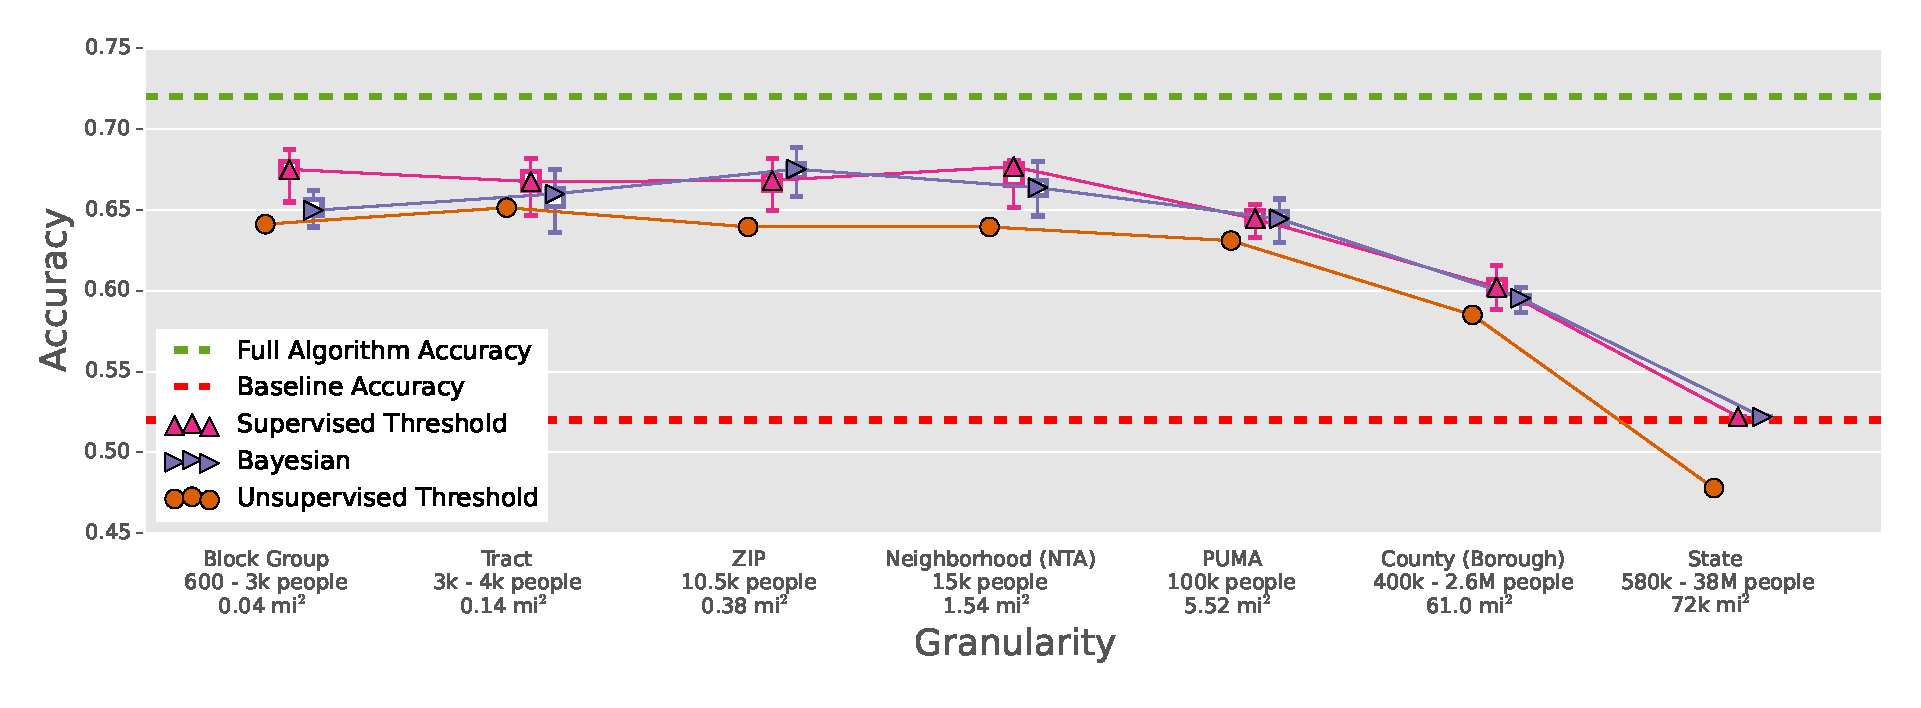
\includegraphics[width=\textwidth]{fig/granularity_plot_both_baselines.eps}
    \caption{Accuracy of ethnicity prediction versus granularity for our NY population using several different inference techniques. Accuracy increases slightly at the ZIP code and neighborhood granularities and then decreases. Interestingly, the Bayesian algorithm, which uses only counts of visits to locations, performs comparably to the Supervised Threshold algorithm, which uses data on the ethnicity of visited locations.}
    \label{fig:big_plot}
\end{figure*}

A detailed comparison of accuracy as a function of granularity and inference scenario can be seen in Figure~\ref{fig:big_plot}.
Granularity decreases (each location is a larger geographic area) as the X axis increases, and the Y axis corresponds to accuracy.
The color of each line corresponds to a different inference scenario.
The \textbf{Bayesian} algorithm uses just the counts of location visits as features.
This corresponds to a scenario where labels are available but locations are anonymized.
The \textbf{Unsupervised Threshold} algorithm uses \emph{no} labels, but rather averages the percentage of Caucasians (or men/women) living all locations that a user visits, outputting a label based on if this average is below or above the city's mean.
This corresponds to a problem scenario where locations are known but users are not labeled.
% To test if labeled data was necessary to guess ethnicity, we developed a simple decision rule that used no labels. Based on Census data we calculated the average percentage of Caucasians living in all locations that a user visited. If this percentage was over the metropolitan area's average, we predicted that the user was Caucasian. If it was below, we predicted that the user was of a minority ethnicity.
% We called this the \textbf{Unsupervised Threshold} algorithm.
In comparison, the \textbf{Supervised Threshold} algorithm learns a threshold via the labeled data, rather than using the city's mean, corresponding to a scenario where there are some labeled users and ``raw" or lightly anonymized location data that can be linked to the census.
% We compared this algorithm to an algorithm with access to labeled data, which learned an optimal threshold rather than using one derived from publicly available Census data and which we dubbed the \textbf{Supervised Threshold} algorithm.
The dashed lines in the graph correspond to our best performing algorithm and the basline.
% Finally, we compared these algorithms against our best performing algorithm, run with all features at the lowest granularity. We call this the \textbf{Full} algorithm.

A few interesting results can be derived from Figure~\ref{fig:big_plot}.
Unsurprisingly, the performance of all algorithms decreases at the most coarse granularities. 
However, the performance stays remarkably flat up to fairly large granularities, without a significant drop until after the PUMA level of roughly 100,000 people.
Additionally, the performance of the Unsupervised Threshold algorithm, which uses \emph{no} labels, is not far from the other algorihtms.
% This is most likely because the ethnicity distributions of larger regions are closer to the overall distribution of the metropolitan area and provide less information. 
Several algorithms improve in performance at medium granularities, such as ZIP and neighborhood, most likely due to the sparsity of our dataset at the most detailed granularity levels.

% This affected our methodology in a few key ways.
% First, we utilized well-understood, commonly-applied techniques that could easily be employed by anyone with access to mobility data.
% We also used publicly available data-sources. 
% Second, to make our results applicable to other sources of location data beyond Instagram, we did not use features specific to Instagram, such as the social network graph or user-generated descriptions.
% Thus, our work should be viewed as a lower-bound on the accuracy of what can be inferred using location data. 
% Adversaries with access to more detailed auxiliary information, more data about each user (such as a contact list or recent purchases), or more advanced machine learning techniques might achieve better results.

% We considered two questions: (1) Can minorities be distinguished from Caucasians? (2) Can women be distinguished from men?
% We represented users as feature vectors, using three classes of features:
% \textbf{geographic} features, such as counts or percentages of visits to locations; 
% \textbf{semantic} features derived from Foursquare, such as the popularity of visited venues or counts of visits to venues with certain categories like ``Restaurant" or ``Park" (the collection of which we explained in \S\ref{sec:method}); 
% and \textbf{Census} derived features, such as the average ethnic makeup of all visited locations or the ethnic makeup of a user's most-visited location.

% We performed all our experiments using the scikit-learn library~\cite{scikit-learn} and tested the algorithms logistic regression, decision trees, naive Bayes, and support vector machines (SVMs). 
% As a baseline, we predicted ethnicity or gender based on the class distribution, giving us baseline accuracies of 52\% for ethnicity in NY, 50\% for ethnicity in LA, and 53\% for gender in NY. 

% \paragraph{Auxiliary Data}

% Auxiliary information about a location derived from Foursquare or the Census may not always be available, e.g., in countries without publicly available census data or when locations are anonymized. 
% Furthermore, a labeled training set of user data may not always be available either. 
% To understand the performance of an algorithm that does not have access to any data beyond counts of visits to locations, we applied our \textbf{Bayesian} algorithm to our data.
% To test if labeled data was necessary to guess ethnicity, we developed a simple decision rule that used no labels. Based on Census data we calculated the average percentage of Caucasians living in all locations that a user visited. If this percentage was over the metropolitan area's average, we predicted that the user was Caucasian. If it was below, we predicted that the user was of a minority ethnicity.
% We called this the \textbf{Unsupervised Threshold} algorithm.
% We compared this algorithm to an algorithm with access to labeled data, which learned an optimal threshold rather than using one derived from publicly available Census data and which we dubbed the \textbf{Supervised Threshold} algorithm.
% Finally, we compared these algorithms against our best performing algorithm, run with all features at the lowest granularity. We call this the \textbf{Full} algorithm.

% \paragraph{Data Granularity}
% The granularity of location data can vary greatly depending on how it is created. %For example, the GPS in a cell phone may have accuracy up to a few yards, while CDR data may cover several square miles. 
% Previous research has investigated the impact of location granularity on anonymity~\cite{de2013unique, Zang:2011hk}. 
% To investigate the impact of granularity on inferences, we represented our location data at several different granularities defined by the Census ranging from block groups to states.
% %For example, in our supervised threshold algorithm, we might use the average ethnicity of the visited counties, as opposed to visited city blocks.
% The ethnic makeup of a large granularity area, such as a county, will typically be more similar to the overall metropolitan area's ethnic makeup than a small granularity area like a city block. Thus, increasing the granularity should make inferences more difficult.



\paragraph{Impact of Data Quantity and Diversity}
% \paragraph{Data Quantity}
Finally, with four different analyses, we studied the impact of data quantity on prediction accuracy.
We examine algorithm accuracy on users grouped according to their number of geolocated Instagram photos and unique ZIP codes.
Both of these are impacted by choices made by users---users who post more might be inherently easier to identify or predict.
We thus did two more analyses where we sampled locations from a user's full set of checkins.
In the first, we ran the Supervised Threshold algorithm on a user's $k$ most visited locations.
In the second, we ran the Supervised Threshold algorithm on $n$ randomly sampled checkins.
The results of this analysis can be seen in~\fig{fig:howmuchdata2}.


% \begin{wrapfigure}{R}{0.5\textwidth}
% % \begin{figure}[h!]
%   \centering
%   % \includegraphics[width=0.49\linewidth]{fig/checkins_to_accuracy.eps}
%   \includegraphics[width=0.49\linewidth]{fig/footprints/checkins_to_accuracy.eps}
%   % \includegraphics[width=0.49\linewidth]{fig/zips_to_accuracy.eps}
%   \includegraphics[width=0.49\linewidth]{fig/footprints/zips_to_accuracy.eps}
%   \caption{Checkin user activity. Left: accuracy as a function of total number of checkins at ZIP code locations. Right: accuracy as a function of number of checkins at distinct ZIP code locations.}
%     \label{fig:howmuchdata}
% % \end{figure}
% \end{wrapfigure}

\begin{figure*}[t]
  \centering
  \includegraphics[width=0.25\linewidth]{fig/footprints/checkins_to_accuracy.eps}
  % \includegraphics[width=0.49\linewidth]{fig/zips_to_accuracy.eps}
  \includegraphics[width=0.25\linewidth]{fig/footprints/zips_to_accuracy.eps}
  % \includegraphics[width=0.49\linewidth]{fig/rand-to-accuracyTract.eps}
  \includegraphics[width=0.24\linewidth]{fig/footprints/rand-to-accuracyTract.eps}
  % \includegraphics[width=0.49\linewidth]{fig/rand-to-accuracyNeighborhood.eps}
  \includegraphics[width=0.24\linewidth]{fig/footprints/rand-to-accuracyNeighborhood.eps}
  \caption{Impact of location quantity and diversity on accuracy. 
  Y axis is accuracy, x axis is (from left to right): 
    (1) Number of checkins used
    (2) Number of unique ZIP codes visited
    (3) Number randomly selected or Top-K Tracts
    (3) Number randomly selected or Top-K Neighborhoods
  % Accuracy of predicting a user's ethnicity from a small number of locations chosen either as most frequently visited locations or randomly. The algorithm used is the Supervised Threshold algorithm. Left: tract granularity. Right: neighborhood granularity.
  }
    \label{fig:howmuchdata2}
\end{figure*}

% In particular, we investigated to what extent a user's total number of checkins and the geographic diversity of those checkins impacted prediction accuracy. We binned users according to how many checkins they made and how many distinct ZIP codes they visited, and then calculated accuracy for each bin. Again, we used five-fold cross validation and 30 different partitionings. Figure~\ref{fig:howmuchdata} shows these results. We compare our Bayesian approach with the highest-performing ``Full" algorithm.

% \subsection{Results}
% \label{subsec:inference-results}

% The results of our best-performing algorithms are displayed in Table~\ref{tab:all-tasks}, and a detailed comparison of accuracy as a function of granularity can be seen in Figure~\ref{fig:big_plot}.
% Our results suggest that geotag data can be used to infer an individual's ethnicity and gender. The accuracy for predicting ethnicity falls squarely within what has been reported for other types of datasets. On the lower bound, in their work of predicting individual Twitter users as African American or not based on linguistic features of Tweets~\cite{ICWSM112886} report as best performance an F-1 score of 0.66. On the upper bound, for predicting whether the ethnic origin of a phone user is inside or outside the United States based on a rich feature set containing Internet usage, call, text message, and location features ~\cite{AltshulerAFEP12} achieved an F-measure of 0.81 and for gender an F-measure of 0.61. For gender~\cite{Zhong:2015:YYG:2684822.2685287} achieved an F-measure of 0.81 for social network users in Beijing and 0.82 for Shanghai based on spatial, temporal, and location context knowledge. Given that our dataset contains far fewer features our results demonstrate that geotags are surprisingly powerful in predicting gender and ethnicity. 

% \paragraph{Auxiliary Data}

% It can be observed in Figure~\ref{fig:big_plot} that the Supervised Threshold algorithm performs much better than the Unsupervised Threshold algorithm suggesting that labeled data improves the algorithmic accuracy across the board by roughly 5\%. Interestingly, the Bayesian algorithm performs comparably to the Supervised Threshold algorithm. Thus, an algorithm with no semantic information about visited locations performs just as well as one that knows the ethnic makeup of all visited locations. This suggests that an adversary with enough location data labeled with demographic data could obtain reasonable levels of accuracy with no knowledge of what locations were visited. Even if locations are ``anonymized," that is, GPS coordinates or venue names were obscured, they can still be used to infer demographic information about the user.

% Another interesting result is that both our Bayesian algorithm and Uninformed algorithm perform well, with the Uninformed algorithm outperforming the Unsupervised Threshold above the neighborhood granularity and the Bayesian algorithm outperforming the supervised threshold. This means that given enough labeled data of counts of visits to locations, an algorithm with no auxiliary information can infer ethnicity with relative good accuracy.

% \paragraph{Data Granularity}
% \label{subsec:inference-granularity}

    % \item \emph{Bayesian}: We tested the simple-hypothesis testing algorithm described in the previous section, which relies on strong assumptions of human mobility.
    % \item \emph{Foursquare}: We ran logistic regression using only the features derived from Foursquare.
    % \item \emph{Full}: The best performing algorithm from \S\ref{subsec:inference-overall} which uses features derived from geography, the US Census, and Foursquare. This serves as an upper bound on performance.

% The Full algorithm (that is, our best performing algorithm, with access to all features at all levels of granularity) achieves the best performance; no algorithm with access to restricted, coarser-grained features is as accurate.
% Comparing this set with our Unsupervised Threshold algorithm shows that auxiliary information provides a large performance boost. However, interestingly, many of the algorithms which only use counts of visits to areas within NY perform as well as the richer features derived from Foursquare. 

% The performance of all algorithms decreases at the most coarse granularities. This is most likely because the ethnicity distributions of larger regions are closer to the overall distribution of the metropolitan area and provide less information. Several algorithms improve in performance at medium granularities, such as ZIP and neighborhood. This is most likely caused by the sparsity of our dataset at the most detailed granularity as many blocks are only visited by a few users.

% \paragraph{Data Quantity}

% It appears that the accuracy of ethnicity prediction improves with the total number of checkins a user has made as shown in Figure~\ref{fig:howmuchdata}. The distinct number of ZIP checkins of a user provides a separate measure of user activity as a user could have a large fraction of checkins in few ZIP codes. We can observe a substantial boost in accuracy after a user checked in at 12 distinct ZIP codes.



%For the Full algorithm we observe a drop in accuracy after 24 ZIP codes, followed by a steady upward trend. 
% While it can be observed that an increase in accuracy generally correlates with increases in total and distinct numbers of ZIP checkins, those variables seem unable to fully explain it. After all, for LA the accuracy decreases until it reaches 79-159 total ZIPs. For NY, users with zero to seven distinct ZIP codes could be predicted more accurately than those having seven to 29. It appears that some ZIP codes increase prediction accuracy better than others.

% In order to explore the individual ZIPs' predictive power we performed two multiple linear regressions---one for NY and one for LA---with the percentage of a ZIP code's inclusion in correct classifications (i.e., the set of correct classifications in which a ZIP code occurs divided by the set of all classifications in which the ZIP code occurs) as the dependent variable and as independent variables (1) the total number of checkins to a ZIP code, (2) the distinct number of users checking in at a ZIP code, and (3) the percentage of Caucasian/minority checkins to a ZIP code. In our regressions we only included ZIP codes that had checkins from at least five distinct users, which left us with 527 different ZIP codes for NY and 207 for LA. 
% 
% We observed that the percentage of Caucasian/minority visits at a ZIP code correlates statistically significantly ($p<0.05$) to its inclusion in the set of correct classifications. Thus, for example, if we have a ZIP code that has 90\% minority checkins and 10\% Caucasian checkins, it was much more likely part of a successful classification than a ZIP code that has equal percentages of minority and Caucasian checkins. The other variables did not prove to be statistically significant. We also tested minority status as independent variable. However, it does not appear to be easier to predict minorities over Caucasians or vice versa.

% We also found that when a user is only observed in a limited set of locations, the inference accuracy increases fast with a relatively small increase in the number of locations. Moreover, it is not even required to focus on the most significant locations of a user to get good inference accuracy. Observations of a user in a few random locations at the tract or neighborhood level might be enough for predicting ethnicity, and those locations may be even selected randomly and must not be necessarily related to the user's most significant places. These results, which are displayed in Figure~\ref{fig:howmuchdata2}, suggest that inference for the purpose of ethnicity identification is quite robust to data sparseness and obfuscation methods.





% ``particularly, heterogeneity holds only for well-off areas. These areas tend to attract people living in areas of varying deprivation. By contrast, Londoners in well off areas do not tend to visit communities that are deprived.''~\cite{conf/pervasive/LathiaQC12}








% \subsection{Inferring Ethnicity and Gender}
% \label{subsec:inference-overall}

% % (1) Using location data, can we predict a user's ethnicity and gender with accuracy better than a random guess? (2) What is the impact of auxiliary information and the granularity of the location data on this prediction? 

% To determine if we could predict the ethnicity and gender of a user with high accuracy, we represented users as feature vectors and tested a number of commonly used machine learning algorithms. We performed all our experiments using the scikit-learn library~\cite{scikit-learn} and tested the algorithms logistic regression, decision trees, naive Bayes, and support vector machines (SVMs). 
% We attempted to distinguish between men and women and turned the question of ethnicity into a binary classification question between Caucasians and minorities. This yielded roughly equal class sizes.

% We used many features, falling into one of three groups: 
% \textbf{general} location-based features, counts or percent of visits to each location; 
% \textbf{Foursquare}-based features such as the average popularity of visited venues or counts of visits to venues with certain categories (the collection of which were mentioned in \S\ref{sec:method}); 
% and \textbf{Census} derived features such as the average ethnic makeup of all visited locations and the ethnic makeup of a user's most-visited location.   
% For each experiment we applied five-fold cross validation, that is, we broke down our data into five groups, trained on four groups, and tested on the remaining group. After running all algorithms with all features, our best results are reported in Table~\ref{tab:all-tasks}. 


% Our results suggest that geotag data can be used to infer an individual's ethnicity and gender. The accuracy for predicting ethnicity falls squarely within what has been reported for other types of datasets. On the lower bound, in their work of predicting individual Twitter users as African-American or not based on linguistic features of Tweets, ~\cite{ICWSM112886} report as best performance an F-1 score of 0.655. On the upper bound, for predicting whether the ethnic origin of a phone user is inside or outside the United States based on a rich feature set containing Internet usage, call, text message, and location features ~\cite{conf/socialcom/AltshulerAFEP12} achieved an F-measure of 0.806 and for gender an F-measure of 0.611. Given that our dataset contains far fewer features our results demonstrate that geotags are surprisingly powerful in predicting ethnicity and gender. 

% \subsection{The Impact of Granularity and Auxiliary Information}
% \label{subsec:inference-granularity}

% \begin{figure*}[htb!]
%   \centering
%   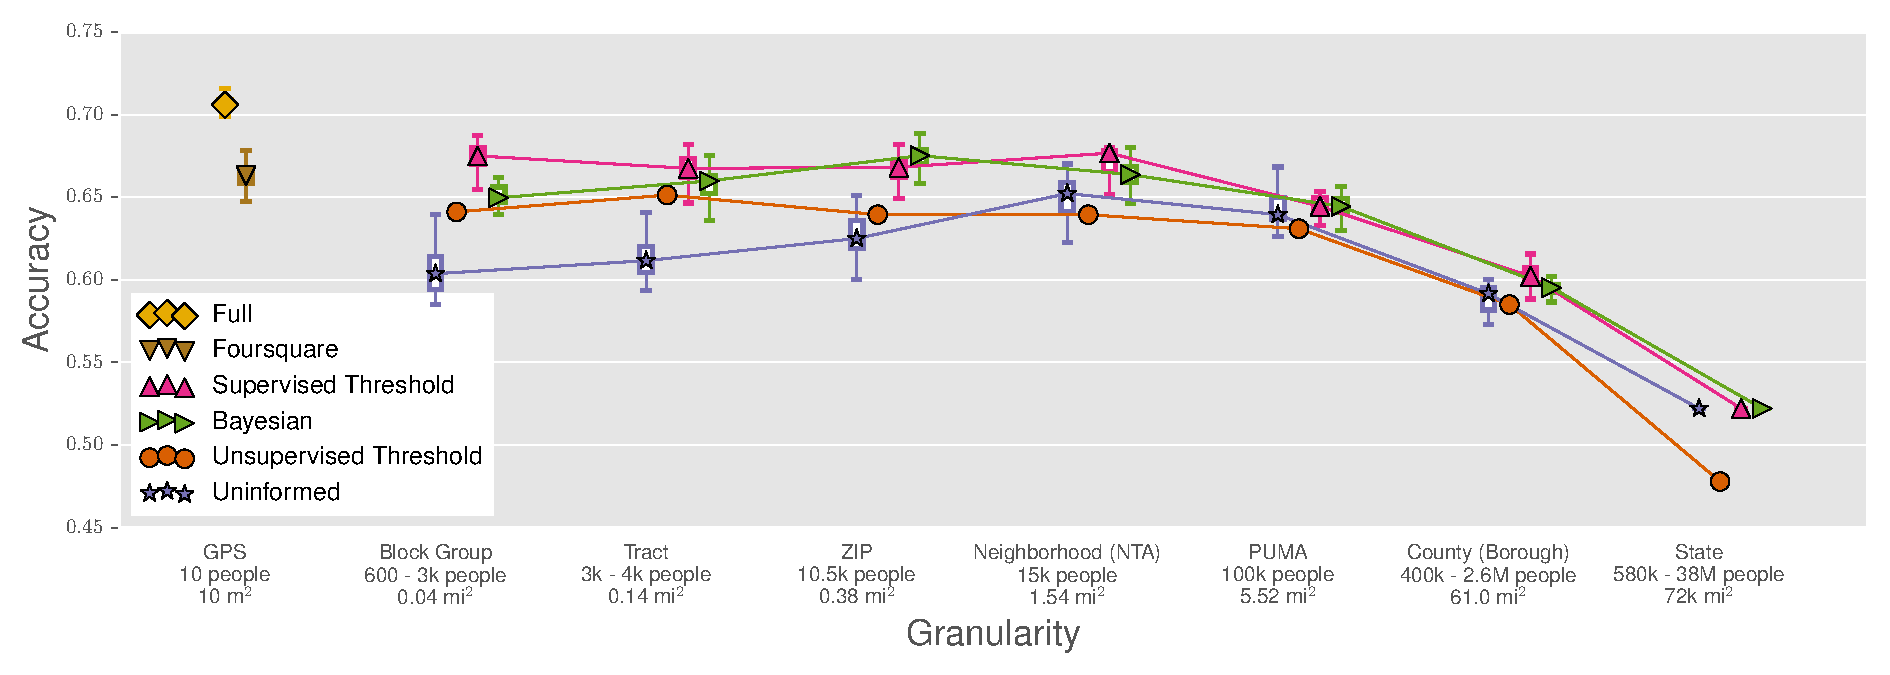
\includegraphics[width=\textwidth]{fig/big_plot_ggplot.pdf}
%   \vspace{0.2ex}
%     \caption{Accuracy of ethnicity prediction versus granularity for our NY population using several different inference techniques. Unsurprisingly, the Full algorithm, which uses features from Foursquare, the US Census, and simple geography, performs the best. Interestingly, however, much simpler algorithms with limited information achieve comparable results.}
%     \label{fig:big_plot}
% \end{figure*}


% Auxiliary information about a location derived from Foursquare or the Census may not always be available, such as in countries without publicly available census data or when locations are anonymized. Additionally, the granularity of location data can vary greatly depending on how it is created. For example, the GPS in a cell phone may have accuracy up to a few yards, while CDR data may cover several square miles. The granularity of location data is often lowered in order to increase the privacy of a dataset. 

% % To study how auxiliary information and granularity impact prediction accuracy we construct feature vectors from the users' sets of visited latitude-longitude locations. We categorize a feature as \emph{informed} if it uses auxiliary information, i.e., census data or Foursquare categories, and as \emph{uninformed} otherwise. In particular, based on census data we computed a threshold by taking the weighted mean of the ethnic distributions for the locations a user visited, and if the user's mean checkin percentage was above the mean for Caucasian visitors, the user was labeled Caucasian and as minority otherwise. Because this method does not require any labeled data, we categorize the resulting features as \emph{unsupervised}. However, other features are \emph{supervised} as they are based on training data labeled by our annotators. 

% In order to understand the impact of auxiliary information and granularity on our ability to make inferences, we compared the highest performing algorithm of \S\ref{subsec:inference-overall} with algorithms that used only a subset of the Foursquare features, Census features, or general features. Additionally, to see if labeled profiles were necessary to infer ethnicity, we tested simple decision rules that required no training.
% % Using different combinations we investigate the following feature sets:
% We employed the following algorithms:

% \begin{itemize}
%     % uninformed supervised features without any auxillary information trained on the percentages of checkins at the various locations.
%     \item \emph{Unsupervised Threshold}: To test if labeled data was necessary to guess ethnicity, we developed a simple decision rule that used no labels. Using census data, we calculated the average percentage of Caucasian people living in all locations that a user visited. If this percentage was over the city's average, we predicted that the user was Caucasian. If it was under, we predicted that the user was a minority.
%     \item \emph{Supervised Threshold}: As a point of comparison, we ran the previously-mentioned decision rule but this time learned the threshold on a set of training data. The performance of this relative to the unsupervised threshold algorithm shows the impact of labeled data.
%     \item \emph{Uninformed}: We ran our best performing algorithm (logistic regression) on a reduced feature set of only the percentages of a user's checkins at each location. This serves as a lower bound on the performance of an algorithm on labeled data using only location information.
%     \item \emph{Bayesian}: We tested the simple-hypothesis testing algorithm described in the previous section, which relies on strong assumptions of human mobility.
%     \item \emph{Foursquare}: We ran logistic regression using only the features derived from Foursquare.
%     \item \emph{Full}: The best performing algorithm from \S\ref{subsec:inference-overall} which uses features derived from geography, the US Census, and Foursquare. This serves as an upper bound on performance.
% \end{itemize}

% We also wanted to understand the impact of location granularity on prediction accuracy. We thus represented our location data at several different granularities defined by the U.S. Census, ranging from block groups to states.
% % , as displayed on the X axis of Figure~\ref{fig:big_plot}.
%  % (600-3,000 individuals) to county (400K- 2.6 million individuals) and state (580K-38 million individuals). 
%  We additionally considered GPS granularity.
%   % (10 individuals).

% For all applicable algorithms, we again employed five-fold cross validation. To view the stability of our algorithms we repeated this process 30 times, using 30 different data partitionings into training and test sets. We ran all algorithms on our dataset of New York City based users.
% The results of this experiment are shown in Figure~\ref{fig:big_plot}.


% % \paragraph{The Impact of Auxillary Information} 
% % \paragraph{The Impact of Granularity}

% It can be observed that the Full algorithm achieves the best performance, as might be expected. Comparing this set with our Uninformed set shows that auxiliary information provides a large performance boost. However, interestingly, many of the algorithms which only use counts of visits to areas within NY perform as well as the richer features derived from Foursquare. Another interesting result is that both our Bayesian algorithm and Uninformed algorithm perform well, with the Uninformed algorithm outperforming the Unsupervised Threshold above the neighborhood granularity and the Bayesian algorithm outperforming the supervised threshold. This means that given enough labeled data of counts of visits to locations, an algorithm with no auxiliary information can infer ethnicity with relative good accuracy.

% The performance of all algorithms decreases at the largest granularities. This is most likely because the ethnicity distributions of larger regions are closer to the overall city distribution and provide less information. Several algorithms improve in performance at medium granularities such as ZIP and Neighborhood. This is most likely caused by the sparsity of our dataset at the highest granularity, as many blocks are visited by only a few users.

% \subsection{The Impact of User Activity}
% \label{sec:user-activity}

% % Finally, we also studied the impact of user activity on prediction accuracy. In particular, we investigated to what extent a user's total number of checkins and the geographic diversity of those checkins impacted prediction accuracy. We binned users according to how many checkins they made and how many distinct ZIP codes they visited, and then calculated accuracy for each bin. Again, we used five-fold cross validation and 30 different partitionings. Figure~\ref{fig:howmuchdata} shows these results. We compare our Bayesian approach with the highest-performing ``Full" algorithm.

% It appears that the accuracy of ethnicity prediction improves with the total number of checkins a user has made. The distinct number of ZIP checkins of a user provides a separate measure of user activity as a user could have a large fraction of checkins in few ZIPs. We can observe a substantial boost in accuracy after a user checked in at 12 distinct ZIP codes. For the Full algorithm we observe a drop in accuracy after 24 ZIP codes, followed by a steady upward trend. 
% % While it can be observed that an increase in accuracy generally correlates with increases in total and distinct numbers of ZIP checkins, those variables seem unable to fully explain it. After all, for LA the accuracy decreases until it reaches 79-159 total ZIPs. For NY, users with zero to seven distinct ZIP codes could be predicted more accurately than those having seven to 29. It appears that some ZIP codes increase prediction accuracy better than others.

% In order to explore the individual ZIPs' predictive power we performed two multiple linear regressions---one for NY and one for LA---with the percentage of a ZIP code's inclusion in correct classifications (i.e., the set of correct classifications in which a ZIP code occurs divided by the set of all classifications in which the ZIP code occurs) as the dependent variable and as independent variables (1) the total number of checkins to a ZIP code, (2) the distinct number of users checking in at a ZIP code, and (3) the percentage of Caucasian/minority checkins to a ZIP code. In our regressions we only included ZIP codes that had checkins from at least five distinct users, which left us with 527 different ZIP codes for NY and 207 for LA. 

% We observed that the percentage of Caucasian/minority visits at a ZIP code correlates statistically significantly ($p<0.05$) to its inclusion in the set of correct classifications. Thus, for example, if we have a ZIP code that has 90\% minority checkins and 10\% Caucasian checkins, it was much more likely part of a successful classification than a ZIP code that has equal percentages of minority and Caucasian checkins. The other variables did not prove to be statistically significant. We also tested minority status as independent variable. However, it does not appear to be easier to predict minorities over Caucasians or vice versa.


% \begin{figure}[h]
%   \centering
%   \includegraphics[width=0.49\linewidth]{fig/checkins_to_accuracy.eps}
%   \includegraphics[width=0.49\linewidth]{fig/zips_to_accuracy.eps}
%   \caption{Checkin user activity. Left: accuracy as a function of total number of checkins at ZIP code locations. Right: accuracy as a function of number of checkins at distinct ZIP code locations.}
%     \label{fig:howmuchdata}
% \end{figure}


% \begin{figure}[h]
%   \centering
%   \includegraphics[width=0.49\linewidth]{fig/rand-to-accuracyTract.eps}
%   \includegraphics[width=0.49\linewidth]{fig/rand-to-accuracyNeighborhood.eps}
%   \caption{}
%     \label{fig:howmuchdata2}
% \end{figure}


% % ``particularly, heterogeneity holds only for well-off areas. These areas tend to attract people living in areas of varying deprivation. By contrast, Londoners in well off areas do not tend to visit communities that are deprived.''~\cite{conf/pervasive/LathiaQC12}
